\documentclass{article}
\usepackage{amsmath}
\usepackage{graphicx}
\usepackage[T1]{fontenc}
\graphicspath{{images/}}
\title{List 2 report}
\author{Albert Kołodziejski}
\begin{document}
\maketitle
\section*{Exercise 1}

\subsection*{Description of problem:}
The point of this exercise is to check what effects have little change in data.

\subsection*{Results:}
For disrupted data, the correct result is equal to -0.004296343192495245.

\begin{center}
    \begin{tabular}{| c | c | c | c |}
        \hline
         & result & error & relative error\\ 
        \hline
        \text{(A)} Float32 & -0.4999443 & 0.49994429944939167 & 4.967e10\\
        \text{(B)} Float32 & -0.4543457 & 0.4543457031149343 & 4.514e10\\
        \text{(C)} Float32 & -0.5 & 0.4999999999899343 & 4.967e10\\
        \text{(D)} Float32 & -0.5 & 0.4999999999899343 & 4.967e10\\
        \hline
        \text{(A)} Float64 & 1.0251881368296672e-10 & 1.1258452438296671e-10 & 11.18 \\
        \text{(B)} Float64 & -1.5643308870494366e-10 & 1.4636737800494365e-10 & 14.54 \\
        \text{(C)} Float64 & 0.0 & 1.0065710699999998e-11 & 1.0 \\
        \text{(D)} Float64 & 0.0 & 1.0065710699999998e-11 & 1.0\\
        \hline
        distorted \text{(A)} Float32& -0.4999443 & 0.4956479562669622 & 115.4 \\
        distorted \text{(B)} Float32& -0.4543457 & 0.4500493599325048 & 104.8\\
        distorted \text{(C)} Float32& -0.5 & 0.4957036568075048 & 115.4\\
        distorted \text{(D)} Float32& -0.5 & 0.4957036568075048 & 115.4\\
        \hline
        distorted \text{(A)} Float64 & -0.004296342739891585 & 4.526036594121319e-10 & 1.053e-7\\
        distorted \text{(B)} Float64 & -0.004296342998713953 & 1.9378129136049527e-10 & 4.510e-8\\
        distorted \text{(C)} Float64 & -0.004296342842280865 & 3.502143800654389e-10 & 8.151e-8\\
        distorted \text{(D)} Float64 & -0.004296342842280865 & 3.502143800654389e-10 & 8.151e-8\\
        \hline
    \end{tabular}
    \end{center}

The distortion that was made resulted in a much better approximation of the correct result. A possible explanation is that because of the change in data, new vectors are less perpendicular, and as a result condition number is smaller.
\newpage
\subsection*{QA:}
\begin{center}
    \textbf{What impact do small changes in data have on results?}
\end{center}
If we treat distortion as an error in input data and compare results to \\
-1.00657107000000e-11 we will see that distored algorithms gave the same results for Float32, and worse results for Float64.
\begin{center}
    \begin{tabular}{| c | c | c | c |}
        \hline
         & result & error & relative error\\ 
        \hline
        \text{(A)} Float32 & -0.4999443 & 0.49994429944939167 & 4.967e10\\
        \text{(B)} Float32 & -0.4543457 & 0.4543457031149343 & 4.514e10\\
        \text{(C)} Float32 & -0.5 & 0.4999999999899343 & 4.967e10\\
        \text{(D)} Float32 & -0.5 & 0.4999999999899343 & 4.967e10\\
        \hline
        \text{(A)} Float64 & 1.0251881368296672e-10 & 1.1258452438296671e-10 & 11.18 \\
        \text{(B)} Float64 & -1.5643308870494366e-10 & 1.4636737800494365e-10 & 14.54 \\
        \text{(C)} Float64 & 0.0 & 1.0065710699999998e-11 & 1.0 \\
        \text{(D)} Float64 & 0.0 & 1.0065710699999998e-11 & 1.0\\
        \hline
        distorted \text{(A)} Float32 & -0.4999443 & 0.49994429944939167 & 4.967e10\\
        distorted \text{(B)} Float32 & -0.4543457 & 0.4543457031149343 & 4.514e10\\
        distorted \text{(C)} Float32 & -0.5 & 0.4999999999899343 & 4.967e10\\
        distorted \text{(D)} Float32 & -0.5 & 0.4999999999899343 & 4.967e10\\
        \hline
        distorted \text{(A)} Float64 & -0.004296342739891585 & 0.004296342729825875 & 4.268e8\\
        distorted \text{(B)} Float64 & -0.004296342998713953 & 0.004296342988648243 & 4.268e8\\
        distorted \text{(C)} Float64 & -0.004296342842280865 & 0.004296342832215154 & 4.268e8\\
        distorted \text{(D)} Float64 & -0.004296342842280865 & 0.004296342832215154 & 4.268e8\\
        \hline
    \end{tabular}
    \end{center}
    introduced error is too small to have any effects on Float32.
    \subsection*{Interpretation and conclusions:}
    This task is badly conditioned because small changes produce big relative disruptions.
\newpage
    \section*{Exercise 2}

\subsection*{Description of problem:}
In this exercise, we will learn why we shouldn't have full trust in visualization software.
\subsection*{Results:}
Desoms:
\begin{center}
    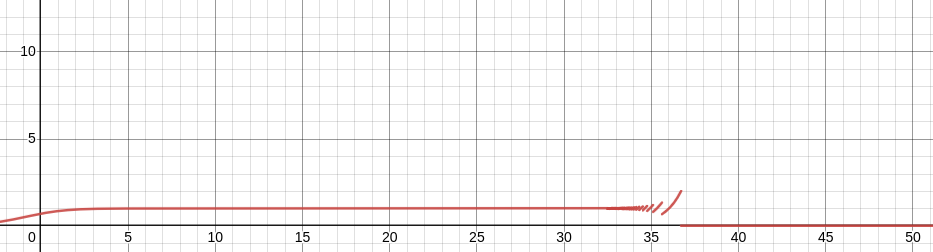
\includegraphics[scale=0.35]{desmos}
\end{center}
WolframAlpha:
\begin{center}
    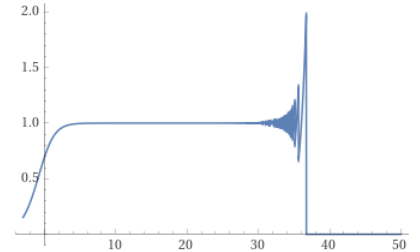
\includegraphics[scale=0.5]{wolfram}
\end{center}
As we can see in both examples function converges to 0, but that's not true. The function should converge to 1:
\[
    \lim_{x\to\infty} e^x ln(1 + e^{-x}) = \lim_{x\to\infty} \frac{ln(1 + e^{-x})}{e^{-x}} = \lim_{x\to\infty} \frac{f(x)}{g(x)}
\]
Both functions are differentiable for real numbers, both f and g are converging to 0 with x going to infinity and the derivative of a function g is non-zero. From L'Hôpital's rule we have got:
\[
    \lim_{x\to\infty} \frac{f(x)}{g(x)} = \lim_{x\to\infty} \frac{f'(x)}{g'(x)} = \lim_{x\to\infty} \frac{-\frac{1}{e^x + 1}}{-e^{-x}} = \lim_{x\to\infty} \frac{1}{1 + e^{-x}} = 1
\]
\newpage
I did some experiments. For x = 1, 2, ..., 40 I have computed e\textsuperscript{-x} + 1:

\begin{center}
    \begin{tabular}{| c | c |}
        \hline
        x & result \\
        \hline
        \hline
        1 & 1.3678794411714423 \\
        \hline
        2 & 1.1353352832366128 \\
        \dots & \dots \\
        34 & 1.0000000000000018 \\
        \hline
        35 & 1.0000000000000007 \\
        \hline
        36 & 1.0000000000000002 \\
        \hline
        37 & 1.0 \\
        \hline
        38 & 1.0 \\
        \hline
        39 & 1.0 \\
        \hline
        40 & 1.0 \\
        \hline

    \end{tabular}
    \end{center}
For x = 37 e\textsuperscript{-x} + 1 = 1, that means ln(e\textsuperscript{-x} + 1) = 0. What explains why on visualisation function converged to 0. Behavior near x = 35 is caused by adding a small number to 1, which causes a loss of important information. 
\subsection*{Interpretation and conclusions:}
We can not trust visualization software to compute how the function is converging.
\section*{Exercise 3}
\subsection*{Description of problem:}
In this exercise, we test how different matrixes will affect the result of simple computation.

\subsection*{Results:}
\begin{center}
    \begin{tabular}{| c | c | c | c | c |}
        \hline
        matrix & rank  & cond & relative error A\textbackslash b & relative error A\textsuperscript{-1}b \\
        \hline
        \hline
        hilb(2) & 2 & 19.28 & 5.661e-16 & 1.124e-15\\
        hilb(3) & 3 & 524.1 & 8.023e-15 & 9.826e-15\\
        hilb(4) & 4 & 15510.0 & 4.452e-13 & 2.95e-13\\
        hilb(5) & 5 & 476600.0 & 1.683e-12 & 8.5e-12\\
        hilb(6) & 6 & 1.495e7 & 2.619e-10 & 3.347e-10\\
        hilb(7) & 7 & 4.754e8 & 1.261e-8 & 5.164e-9\\
        hilb(8) & 8 & 1.526e10 & 1.027e-7 & 2.699e-7\\
        hilb(9) & 9 & 4.932e11 & 4.832e-6 & 9.176e-6\\
        hilb(10) & 10 & 1.602e13 & 0.0006329 & 0.0004552\\
        hilb(11) & 10 & 5.223e14 & 0.01154 & 0.008044\\
        hilb(12) & 11 & 1.752e16 & 0.2976 & 0.3439\\
        hilb(13) & 11 & 3.188e18 & 2.375 & 5.586\\
        hilb(14) & 11 & 6.201e17 & 5.281 & 4.801\\
        hilb(15) & 12 & 3.676e17 & 1.177 & 4.827\\
        hilb(16) & 12 & 7.046e17 & 20.56 & 31.74\\
        hilb(17) & 12 & 1.249e18 & 17.74 & 15.91\\
        hilb(18) & 12 & 2.248e18 & 41.48 & 33.88\\
        hilb(19) & 13 & 6.473e18 & 101.7 & 94.41\\
        hilb(20) & 13 & 1.148e18 & 6.505 & 71.95\\
        \hline
        matcond(5, 1.0) & 5 & 1.0 & 4.965e-17 & 1.57e-16\\
        matcond(5, 10.0) & 5 & 10.0 & 1.986e-16 & 4.578e-16\\
        matcond(5, 1000.0) & 5 & 1000.0 & 3.186e-14 & 2.493e-14\\
        matcond(5, 1.0e7) & 5 & 1.0e7 & 2.154e-11 & 6.403e-11\\
        matcond(5, 1.0e12) & 5 & 1.0e12 & 7.469e-6 & 3.394e-6\\
        matcond(5, 1.0e16) & 4 & 9.577e15 & 0.02785 & 0.04316\\
        matcond(10, 1.0) & 10 & 1.0 & 1.955e-16 & 3.237e-16\\
        matcond(10, 10.0) & 10 & 10.0 & 3.458e-16 & 2.164e-16\\
        matcond(10, 1000.0) & 10 & 1000.0 & 1.862e-14 & 1.674e-14\\
        matcond(10, 1.0e7) & 10 & 1.0e7 & 2.411e-10 & 2.251e-10\\
        matcond(10, 1.0e12) & 10 & 1.0e12 & 1.352e-5 & 1.492e-5\\
        matcond(10, 1.0e16) & 9 & 1.353e16 & 0.4888 & 0.5268\\
        matcond(20, 1.0) & 20 & 1.0 & 3.933e-16 & 4.041e-16\\
        matcond(20, 10.0) & 20 & 10.0 & 3.169e-16 & 3.312e-16\\
        matcond(20, 1000.0) & 20 & 1000.0 & 1.252e-14 & 8.917e-15\\
        matcond(20, 1.0e7) & 20 & 1.0e7 & 2.076e-10 & 1.879e-10\\
        matcond(20, 1.0e12) & 20 & 1.0e12 & 5.835e-5 & 5.734e-5\\
        matcond(20, 1.0e16) & 19 & 2.025e16 & 0.133 & 0.163\\
        \hline
    \end{tabular}
    \end{center}

\subsection*{Interpretation and conclusions:}
The relative error is highly correlated with the condition number of the matrix, and the rank computed in float arithmetic isn't always equal mathematical rank.
\newpage
\section*{Exercise 4}
\subsection*{Description of problem:}
In this exercise, we are testing the Wilkinson polynomial.

\subsection*{Results:}
\begin{center}
    \begin{tabular}{| c | c | c | c | c |}
        \hline
        k & z & |P(z)| & |p(z)| & |z - k|\\
        \hline
        1 & 0.9999999999996989 & 35700.0 & 36630.0 & 3.011e-13\\
        2 & 2.0000000000283182 & 176300.0 & 181300.0 & 2.832e-11\\
        3 & 2.9999999995920965 & 279200.0 & 290200.0 & 4.079e-10\\
        4 & 3.9999999837375317 & 3.027e6 & 2.042e6 & 1.626e-8\\
        5 & 5.000000665769791 & 2.292e7 & 2.089e7 & 6.658e-7\\
        6 & 5.999989245824773 & 1.29e8 & 1.125e8 & 1.075e-5\\
        7 & 7.000102002793008 & 4.805e8 & 4.573e8 & 0.000102\\
        8 & 7.999355829607762 & 1.638e9 & 1.556e9 & 0.0006442\\
        9 & 9.002915294362053 & 4.877e9 & 4.688e9 & 0.002915\\
        10 & 9.990413042481725 & 1.364e10 & 1.263e10 & 0.009587\\
        11 & 11.025022932909318 & 3.586e10 & 3.3e10 & 0.02502\\
        12 & 11.953283253846857 & 7.533e10 & 7.389e10 & 0.04672\\
        13 & 13.07431403244734 & 1.961e11 & 1.848e11 & 0.07431\\
        14 & 13.914755591802127 & 3.575e11 & 3.551e11 & 0.08524\\
        15 & 15.075493799699476 & 8.216e11 & 8.423e11 & 0.07549\\
        16 & 15.946286716607972 & 1.551e12 & 1.571e12 & 0.05371\\
        17 & 17.025427146237412 & 3.695e12 & 3.317e12 & 0.02543\\
        18 & 17.99092135271648 & 7.65e12 & 6.345e12 & 0.009079\\
        19 & 19.00190981829944 & 1.144e13 & 1.229e13 & 0.00191\\
        20 & 19.999809291236637 & 2.792e13 & 2.318e13 & 0.0001907\\
        \hline
    \end{tabular}
    \end{center}

    \subsection*{QA:}
\begin{center}
    \textbf{Can you explain discrepancies?}
\end{center}
In the formula, we have got big powers, which cause loss of information, and because this task is badly conditioned small changes in data will cause huge changes in result.
\newpage
\begin{center}
    \textbf{Can you repeat Wilkinson experiment?}
\end{center}
In this experiment, Wilkinson subtracted 2\textsuperscript{-23} from -210 in the formula and showed that the new polynomial has complex roots.

\begin{center}
    \begin{tabular}{| c | c | c | c | c |}
        \hline
        k & z & |P(z)| & |p(z)| & |z - k|\\
        \hline
        1 & 0.9999999999998357 + 0.0im & 20260.0 & 19990.0 & 1.643e-13\\
2 & 2.0000000000550373 + 0.0im & 346500.0 & 352400.0 & 5.504e-11\\
3 & 2.99999999660342 + 0.0im & 2.366e6 & 2.416e6 & 3.397e-9\\
4 & 4.000000089724362 + 0.0im & 1.002e7 & 1.126e7 & 8.972e-8\\
5 & 4.99999857388791 + 0.0im & 4.625e7 & 4.476e7 & 1.426e-6\\
6 & 6.000020476673031 + 0.0im & 2.024e8 & 2.142e8 & 2.048e-5\\
7 & 6.99960207042242 + 0.0im & 1.711e9 & 1.785e9 & 0.0003979\\
8 & 8.007772029099446 + 0.0im & 1.87e10 & 1.869e10 & 0.007772\\
9 & 8.915816367932559 + 0.0im & 1.376e11 & 1.375e11 & 0.08418\\
10 & 10.095455630535774 - 0.6449328236240688im & 1.491e12 & 1.49e12 & 0.652\\
11 & 10.095455630535774 + 0.6449328236240688im & 1.491e12 & 1.49e12 & 1.111\\
12 & 11.793890586174369 - 1.6524771364075785im & 3.297e13 & 3.296e13 & 1.665\\
13 & 11.793890586174369 + 1.6524771364075785im & 3.297e13 & 3.296e13 & 2.046\\
14 & 13.992406684487216 - 2.5188244257108443im & 9.546e14 & 9.546e14 & 2.519\\
15 & 13.992406684487216 + 2.5188244257108443im & 9.546e14 & 9.546e14 & 2.713\\
16 & 16.73074487979267 - 2.812624896721978im & 2.742e16 & 2.742e16 & 2.906\\
17 & 16.73074487979267 + 2.812624896721978im & 2.742e16 & 2.742e16 & 2.825\\
18 & 19.5024423688181 - 1.940331978642903im & 4.253e17 & 4.252e17 & 2.454\\
19 & 19.5024423688181 + 1.940331978642903im & 4.253e17 & 4.252e17 & 2.004\\
20 & 20.84691021519479 + 0.0im & 1.374e18 & 1.374e18 & 0.8469\\
        \hline
    \end{tabular}
    \end{center}
As we can see there are complex roots, what's more 10 and 11 are only different on the imaginary part of a number. That is also true for 12 and 13, 14 and 15, 15 and 17, 18 and 19. It has also resulted in worse results.

\subsection*{Interpretation and conclusions:}
We have to be careful when dealing with Wilkinson polynomials. It is really sensitive to little changes.
\newpage
\section*{Exercise 5}
\subsection*{Description of problem:}
In this exercise, we are experimenting with recursive formula, by computing it in Float32, Float64 and Float32 but with truncation to the 3rd digit after the decimal point on the 10th iteration.

\subsection*{Results:}
\begin{center}
    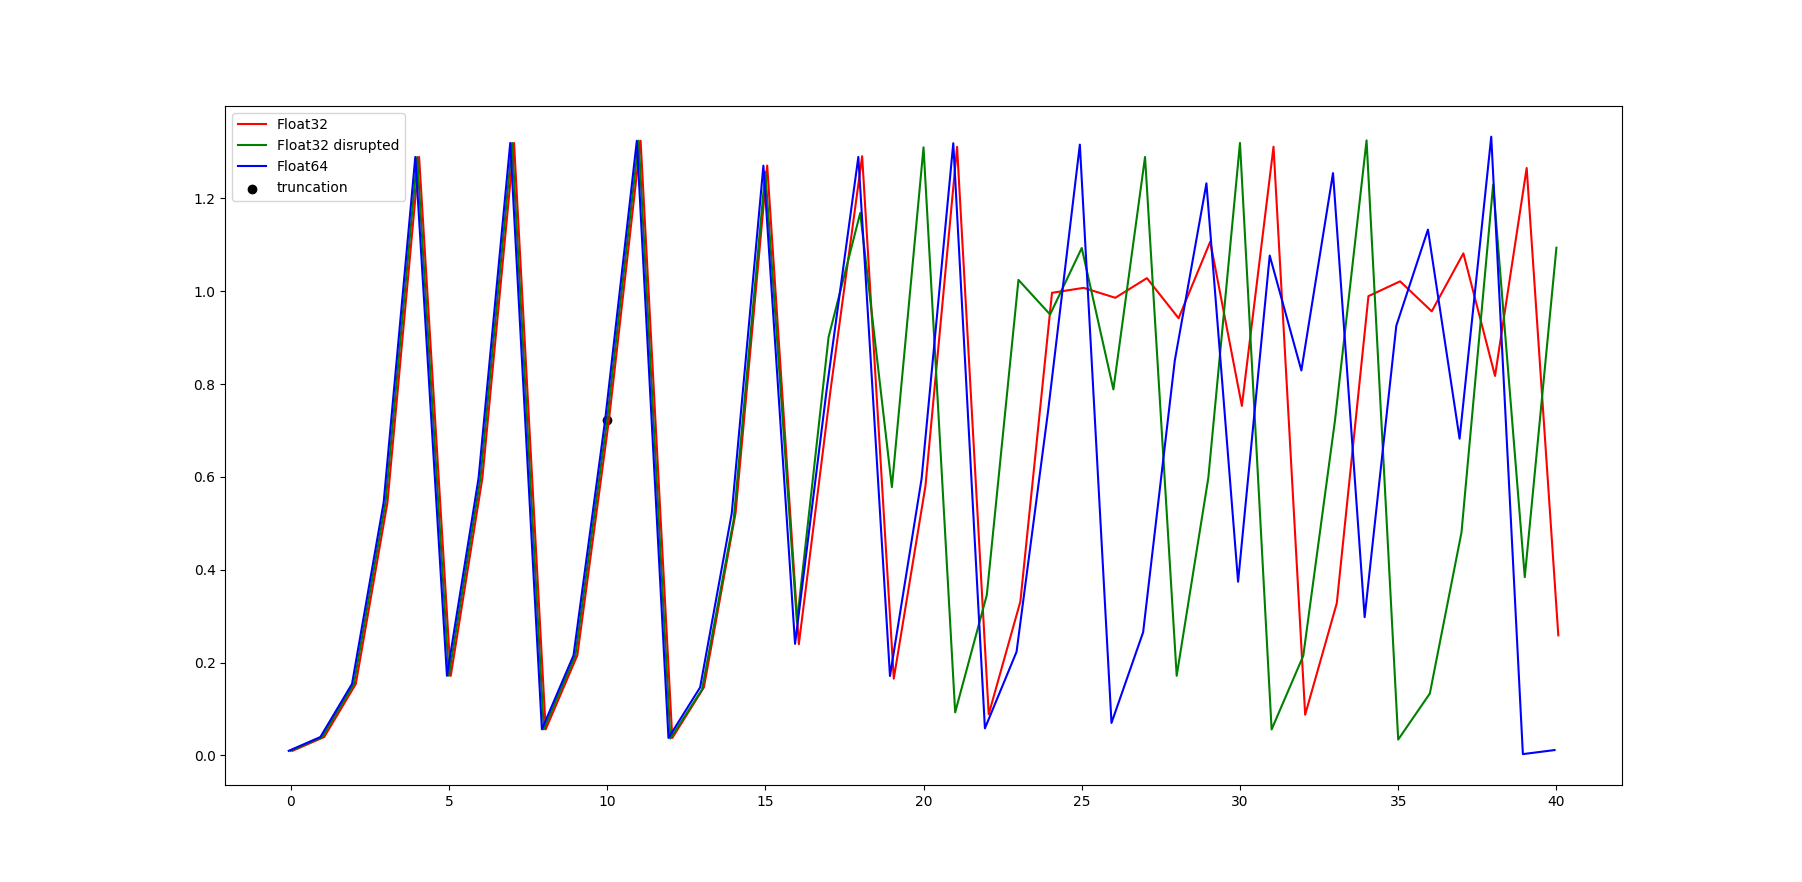
\includegraphics[scale=0.37]{chaos}
\end{center}
 Although at the beginning they are all close to each other, small errors sum up causing big changes in late iterations.

 \subsection*{Interpretation and conclusions:}
Prediction of far future is really hard, small meaningless errors at the beginning lead to chaos after some time.
\newpage
\section*{Exercise 6}
\subsection*{Description of problem:}
In this exercise we are making an experiment testing the recursive formula:
\[
    x\textsubscript{n + 1} := x\textsubscript{n}^{2} + c
\]

\subsection*{Results:}

\begin{center}
    \textbf{c = -2, x\textsubscript{0} = 1}
    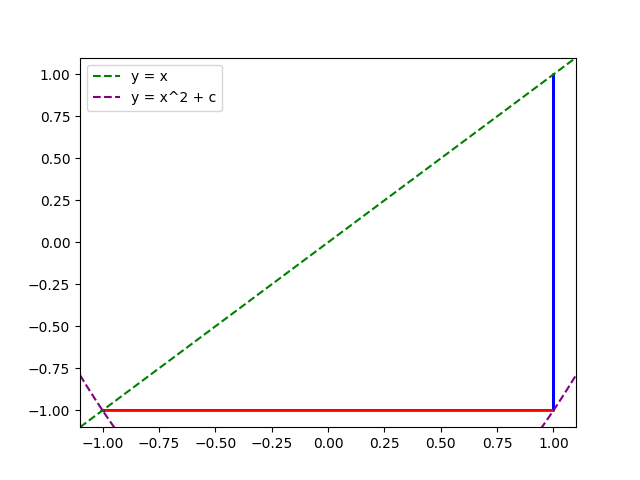
\includegraphics[scale=0.8]{1}
        \begin{tabular}{| c | c |}
            \hline
            n & x\\
            \hline
            0 & 1\\
            1 & -1\\
            2 & -1 \\
            \dots & \dots \\
            39 & -1\\
            40 & -1\\
            \hline
        \end{tabular}
        \end{center}

In the first iteration formula reached a stable point:
\[
    f(1) = 1^{2} - 2 = 1 - 2 = -1 
\]
\[
    f(-1) = -1^{2} - 2 = 1 - 2 = -1 
\]
\newpage
\begin{center}
    \textbf{c = -2, x\textsubscript{0} = 2}
    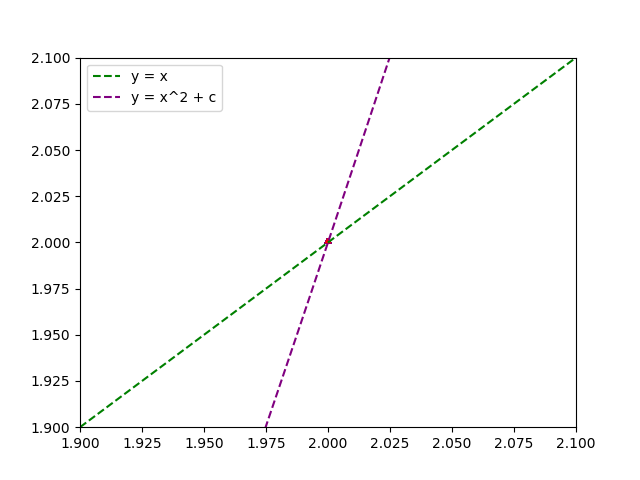
\includegraphics[scale=0.8]{2}
    \begin{tabular}{| c | c |}
        \hline
        n & x\\
        \hline
        0 & 2\\
        1 & 2\\
        2 & 2 \\
        \dots & \dots \\
        39 & 2\\
        40 & 2\\
        \hline
    \end{tabular}
    \end{center}

The formula starts from a stable point:
\[
f(2) = 2^{2} - 2 = 4 - 2 = 2 
\]

\newpage
\begin{center}
    \textbf{c = -2, x\textsubscript{0} = 1.99999999999999}
    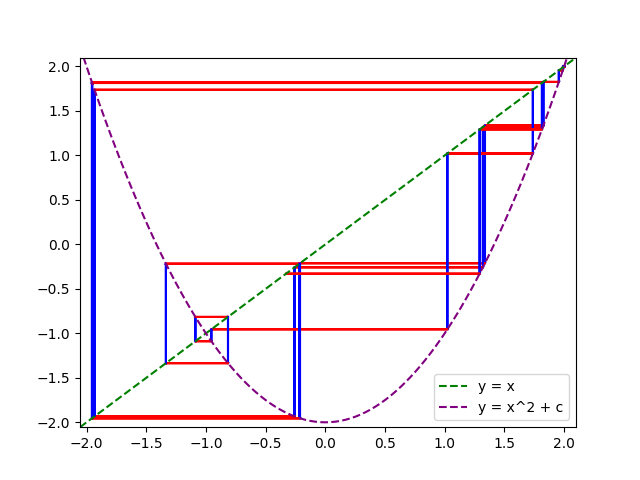
\includegraphics[scale=0.8]{3}
    \begin{tabular}{| c | c |}
        \hline
        n & x\\
        \hline
        0 & 1.99999999999999\\
        1 & 1.99999999999996\\
        \dots & \dots \\
        21 & 1.9562153843260486 \\
        \hline
        22 & 1.82677862987391 \\
        23 & 1.3371201625639997\\
        24 & -0.21210967086482313\\
        25 &-1.9550094875256163\\
        \hline
        26 & 1.822062096315173\\
        27 & 1.319910282828443\\
        28 & -0.2578368452837396\\
        29 & -1.9335201612141288\\
        \hline
        30 & 1.7385002138215109\\
        31 &  1.0223829934574389\\
        32 &  -0.9547330146890065\\
        \dots & \dots \\
        \hline
    \end{tabular}
    \end{center}
For the first 20 iterations, it is slowly going away from x = 2, then it goes into a 4-point cycle (1.8, 1.3, -0.2, -1.9) just to go close to stable point -1 and spirals away from it and do one last 4-point cycle. There could be some more stable pattern that isn't possible due to floating point errors.

\newpage
\begin{center}
    \textbf{c = -1, x\textsubscript{0} = 1}
    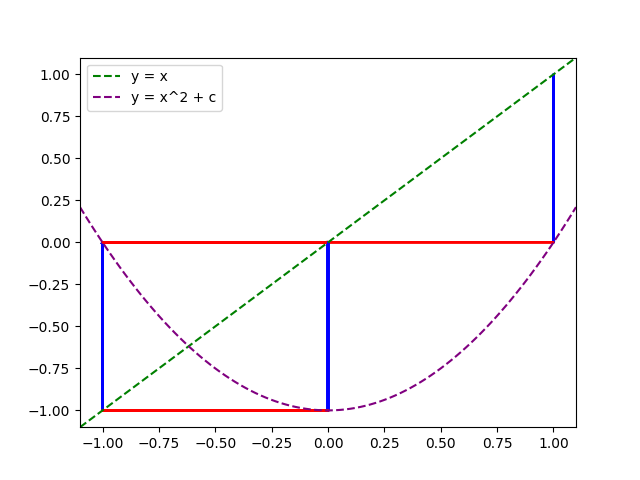
\includegraphics[scale=0.8]{4}
    \begin{tabular}{| c | c |}
        \hline
        n & x\\
        \hline
        0 & 1\\
        1 & 0\\
        2 & -1\\
        3 & 0\\
        \dots & \dots \\ 
        39 & 0\\
        40 &  -1\\
        \hline
    \end{tabular}
    \end{center}
The formula ends up in a stable 2-point cycle:
\[
f(1) = 1^{2} - 1 = 1 - 1 = 0 
\]
\[
f(0) = 0^{2} - 1 = 0 - 1 = -1 
\]
\[
f(-1) = -1^{2} - 1 = 1 - 1 = 0 
\]

\newpage
\begin{center}
    \textbf{c = -1, x\textsubscript{0} = -1}
    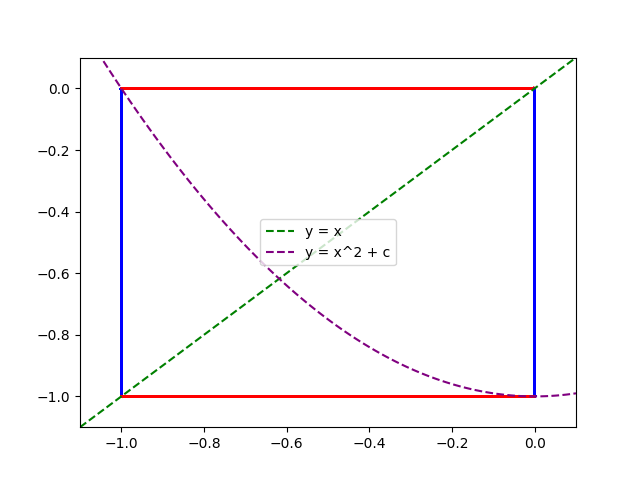
\includegraphics[scale=0.8]{5}
    \begin{tabular}{| c | c |}
        \hline
        n & x\\
        \hline
        0 & -1\\
        1 & 0\\
        2 & -1\\
        3 & 0\\
        \dots & \dots \\ 
        39 & 0\\
        40 &  -1\\
        \hline
    \end{tabular}
    \end{center}
The formula starts in a stable 2-point cycle:
\[
f(-1) = -1^{2} - 1 = 1 - 1 = 0 
\]
\[
f(0) = 0^{2} - 1 = 0 - 1 = -1 
\]

\newpage
\begin{center}
    \textbf{c = -1, x\textsubscript{0} = 0.75}
    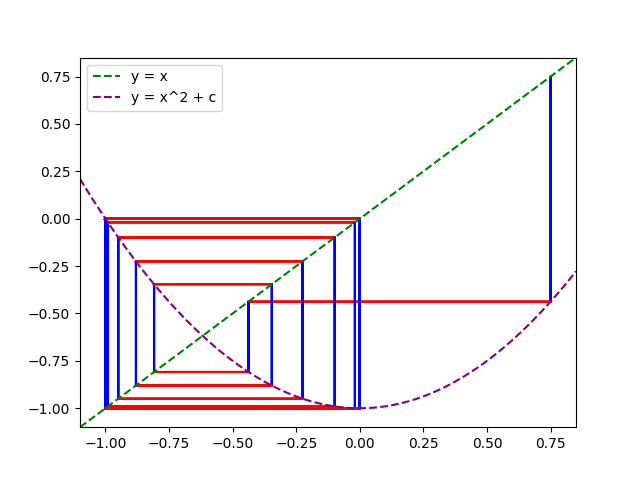
\includegraphics[scale=0.8]{6}
    \begin{tabular}{| c | c |}
        \hline
        n & x\\
        \hline
        0 & 0.75\\
        1 & -0.4375\\
        2 & -0.80859375\\ 
        3 & -0.3461761474609375\\
        \dots & \dots \\ 
        37 & 0\\
        38 &  -1\\
        39 & 0\\
        40 &  -1\\
        \hline
    \end{tabular}
    \end{center}
The formula quickly goes into a spiral and makes its way out into a stable 2-point cycle:
\[
f(-1) = -1^{2} - 1 = 1 - 1 = 0 
\]
\[
f(0) = 0^{2} - 1 = 0 - 1 = -1 
\]
\newpage
\begin{center}
    \textbf{c = -1, x\textsubscript{0} = 0.25}
    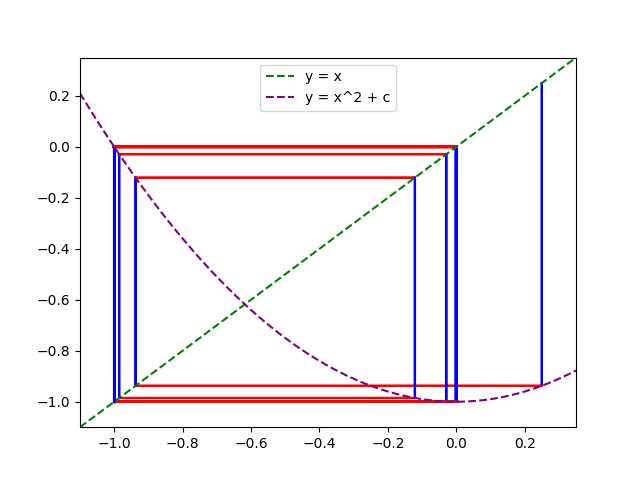
\includegraphics[scale=0.8]{7}
    \begin{tabular}{| c | c |}
        \hline
        n & x\\
        \hline
        0 & 0.25\\
        1 & -0.9375\\
        2 & -0.12109375\\ 
        3 & -0.9853363037109375\\
        \dots & \dots \\ 
        37 & -1\\
        38 &  0\\
        39 & -1\\
        40 &  0\\
        \hline
    \end{tabular}
    \end{center}
    The formula quickly goes into a spiral and makes its way out into a stable 2-point cycle:
    \[
    f(-1) = -1^{2} - 1 = 1 - 1 = 0 
    \]
    \[
    f(0) = 0^{2} - 1 = 0 - 1 = -1 
    \]

 \subsection*{Interpretation and conclusions:}
Recursive formulas can have a wide range of behaviors, like going into a stable point or in a stable cycle.
\end{document}